\subsubsection{Impressió dels gràfics}

\paragraph{}
A causa del funcionament de la funcionalitat, resulta fàcil, que a la mínima que es realitza una cerca mitjanment gran, aquesta tardi més d'un minut en completar-se.

Per tal de transmetre sensació de moviment i que el sistema està treballant, hem introduït a la funcionalitat la capacitat d'anar pintant els gràfics de cada any, a mesura que les dades van quedant disponibles. És a dir, que no cal esperar fins al final de la cerca, per poder començar a explorar elsresultats.

Per aconseguir aquest efecte, disposem de variables globals que comptabilitzen el nombre de cerques que ja han retornat del SDK i cada cop que les dades d'un any queden completades, es pinta el mapa geogràfic i el gràfic de barres, relatiu a l'any. Un cop es completen les dades de tots els anys, es pinta el gràfic de línies.

Els gràfics es pinten mitjançant la crida a l'API de GoogleCharts. Per pintar qualsevol gràfic, sempre se segueix un procés similar:

\begin{enumerate}
    \item Transformació de les dades a un format que Google utilitzarà després per crear el gràfic.
    \item Creació del tipus de gràfic desitjat mitjançant una crida a l'API de Google i selecció del contenidor HTML en el qual volem inserir el gràfic.
    \item Renderització del gràfic en el HTML.
\end{enumerate}

Pel mapa geogràfic, gràcies a la forma en què s’han anat emmagatzemant les dades, el procés és relativament simple. Recordem, que cada fila de la matriu \emph{geomap\-Countries}, representa els valors d’un any i cada columna, un país diferent.

\begin{lstlisting}[style=rawOwn,caption={Creació del mapa geogràfic}]
function printGeomap(i) {
    var geomapData = google.visualization.arrayToDataTable(geomapCountries[i]);
    geomap = new google.visualization.GeoChart(document.getElementById(`geomap'));
    geomap.draw(geomapData, geomapOptions);
}
\end{lstlisting}

Per pintar el gràfic de barres, el procés és molt similar al del mapa geogràfic, però primer realitzem un petit tractament de les dades, per tal d'ordenar els països de més a menys instàncies trobades i obtenir així, una representació més clara de la resposta.

Per aconseguir-ho, es crea una funció de comparació dedicada (\emph{compare\-Countries}), que compararà els diferents elements de l'objecte \emph{barchartCountries}, a través de la funció \emph{sort} pròpia de Javascript.

\begin{lstlisting}[style=rawOwn,caption={Creació del gràfic de barres}]
function compareCountries(a, b) {
    if(parseInt(a[1]) < parseInt(b[1])) return 1;
    else if(parseInt(a[1]) > parseInt(b[1])) return -1;
    else return 0;
}

function printBarchart(i) {
    // Sort data
    var barchartCountries = geomapCountries[i];
    var first = barchartCountries.splice(0, 1);
    barchartCountries.sort(compareCountries);
    barchartCountries.unshift(first[0]);

    // transform and plot
    var barchartData = google.visualization.arrayToDataTable(barchartCountries);
    barchart = new google.charts.Bar(document.getElementById(`barchart'));
    barchart.draw(barchartData, barchartOptions);
}
\end{lstlisting}

En últim lloc, el gràfic de línies també resulta bastant fàcil de pintar, ja que gràcies a la forma en què s’han emmagatzemat les dades, no fa falta realitzar cap tractament especial sobre aquestes, abans de pintar-les.

\begin{lstlisting}[style=rawOwn,caption={Creació del gràfic de línies}]
function printLinechart() {
    ...
    linechartData.addRows(linechartRows);
    linechart = new google.charts.Line(document.getElementById(`linechart'));
    linechart.draw(linechartData, linechartOptions);
    ...
}
\end{lstlisting}

Les figures~\ref{fig:geomap}, \ref{fig:barchart} i \ref{fig:linechart}, ofereixen una visualització dels diferents gràfics disponibles.

\begin{figure}[h]
    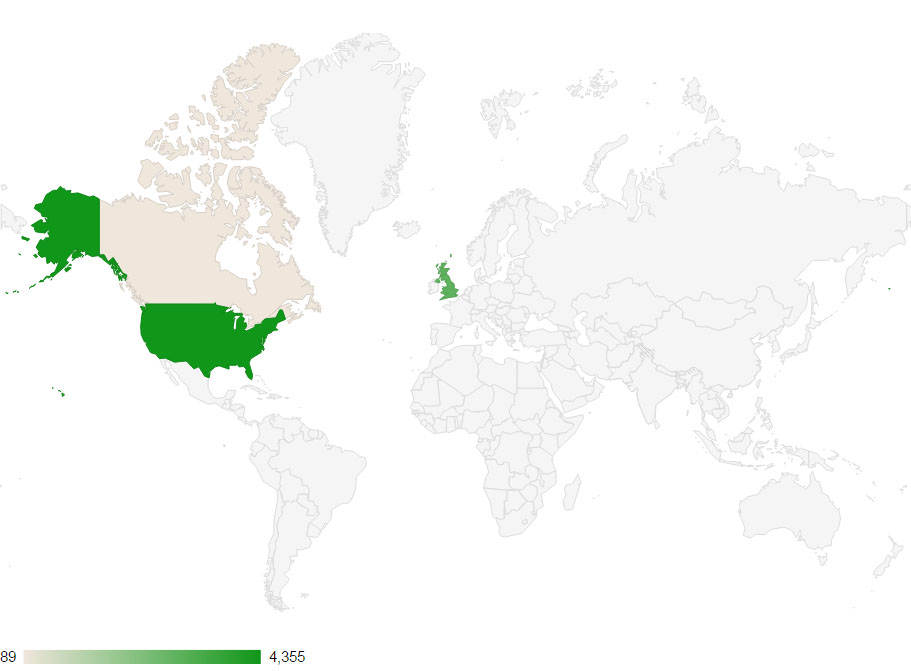
\includegraphics[width=\linewidth]{11/03_surnamesSearch/02_geomapDesktop2}
    \centering
    \caption{Mapa geogràfic}\label{fig:geomap}
\end{figure}

\begin{figure}[h]
    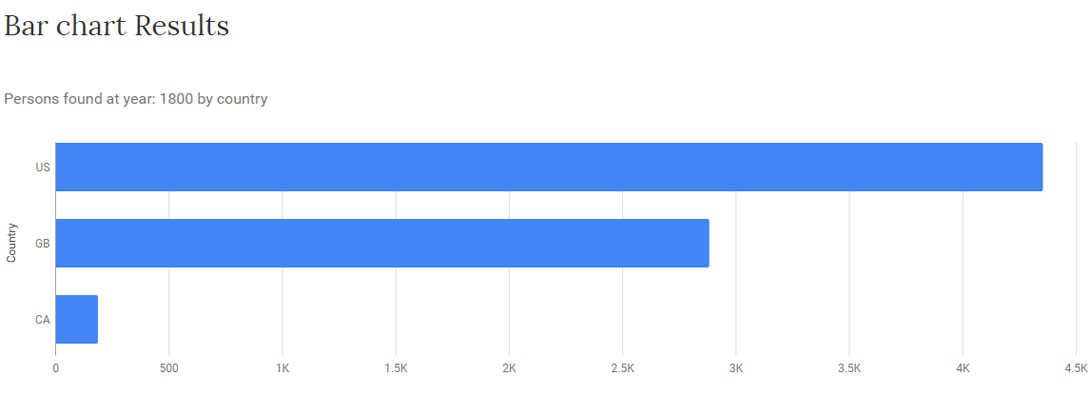
\includegraphics[width=\linewidth]{11/03_surnamesSearch/03_barChartDesktop2}
    \centering
    \caption{Gràfic de barres}\label{fig:barchart}
\end{figure}

\begin{figure}[h]
    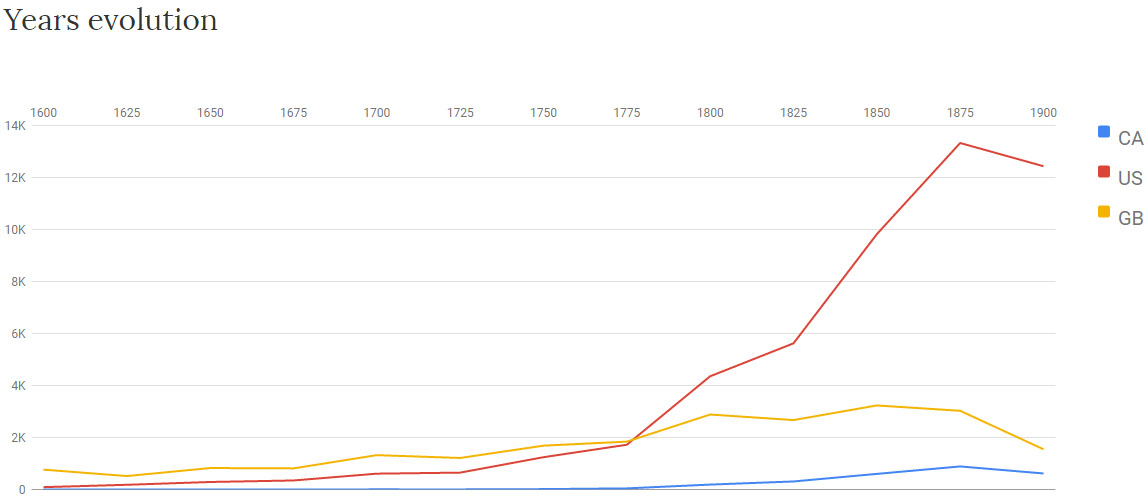
\includegraphics[width=\linewidth]{11/03_surnamesSearch/04_yearsEvolutionDesktop3}
    \centering
    \caption{Gràfic de línies}\label{fig:linechart}
\end{figure}
